\documentclass[a4paper]{article}

\usepackage{fullpage} % Package to use full page
\usepackage{parskip} % Package to tweak paragraph skipping
\usepackage{tikz} % Package for drawing
\usepackage{amsmath}
\usepackage{hyperref}

\title{Image Processing Libraries}
\author{Priyanshu Gautam, Sameer Vivek Pande}
\date{2019/02/16}

\begin{document}

\maketitle

\section{Introduction}

Image processing has been on the rise with the advent of neural networks and machine learning in the past decade. It has therefore become almost absolutely necessary to have image processing libraries to perform convolution, to calculate correlation, linear activations and all the other functions which are the building blocks of any image recognition API. 
In our assignment one, we had to implement this only. In our first subtask we made our own functions for convolution, relu activation, tanh activations, convolution using matrix multiplication, convolution using iteration and so on. In the subtask 2, what we were required to do was to make this process more efficient via exploring \begin{itemize}
\item Already available Linear Algebra libraries having all the optimisation techniques like mkl and openBlas
\item Exploring multi threading for making the process of matrix multiplication parallel and more efficient.
\end {itemize}

In this subtask we shall go through each library and compare their performances on different sets of inputs.

%\begin{figure}[!htbp]
%\begin{center}
%\begin{tikzpicture}
%\draw[domain=-2:2, color=blue] plot (\x, {1 - (\x)^2}) node[above = .5cm, right, color=blue] {$f(x)=1-x^2$};
%\draw[domain=-2:2, color=red] plot(\x,-1 * \x + 1.25) node[above = .5cm, right, color=red] {Tangent at $x=.5$};
%\draw [thick, ->] (-3,0) -- (3,0) node [above] {$x$};
%\draw [thick, ->] (0,-3) -- (0,3) node [right] {$y$};
%\node at (.5,.75) {\textbullet};
%\end{tikzpicture}
%\end{center}
%\caption{The plot of $f(x)=1-x^2$ with a tangent at $x=.5$.} \label{exampleplot}
%\end{figure}


\section{MKL library}

lol \cite{small}
\section{OpenBlas}


\section{Pthread}
To implement multi threading, we made use of pthread module of C++. This allowed us to perform parallel computations in matrix multiplication, as to fully utilise our CPU resources. But for this implementation to be any faster, our number of threads must be equal to the number of cores in the processor, otherwise this technique renders itself to be useless. If number of threads are more, waiting time exists, and the overhead time cost of creating a thread makes the process even slower. Therefore in order to optimise our function we set the number of threads to be 2 which will in most cases decrease the time. For faster time, you can pass the argument as a parameter.
The overhead time cost is negligible for large and small values of filters and inputs but for intermediate values, it becomes considerable enough and the normal multiplication becomes as fast as pthread implementation. It can be seen in the tables \ref{table:nonn} and \ref{table:nonlin} and also in figures \ref{3filter} and \ref{9filter}.


\section{Comparison}
To compare how the publicaly available libraries - mkl, and openBlas, and our multi threading implementation fared against our original matrix multiplication, we did a comparative study of all of these by running them on a random set of inputs.

For doing this comparative study, we calculated the time taken by each of them to multiply two random matrices (one input matrix, and the other kernel), with the size of the input matrix being varied from 32 to 1024, and the size of kernel taken as 3 and 5 for all the input matrices. To calculate the time elapsed we made use of \textbf{high\_resolution\_clock} class present in \textbf{chrono} library. All the data was calculated in seconds, for kernel size of 3, the data is shown in table \ref{table:nonlin} while for the kernel of size 9, it is shown in table \ref{table:nonn}  

\begin{table}[ht]
\caption{Comparative Data for kernel size 3} % title of Table
\centering % used for centering table
\begin{tabular}{c c c c c} % centered columns (4 columns)
\hline\hline %inserts double horizontal lines
Size of input & MKL & OpenBlas & Pthread & Normal \\ [0.5ex] % inserts table
%heading
\hline % inserts single horizontal line
32 & $4.481424\times 10^{-3}$ & $3.480212\times 10^{-3}$ & $3.102635\times 10^{-3}$ & $6.335516\times 10^{-5}$  \\
64 & $3.220144\times 10^{-2}$ & $3.823522\times 10^{-2}$ & $2.418458\times 10^{-3}$ & $2.683123\times 10^{-4}$  \\
128 & $3.878288\times 10^{-2}$ & $4.375075\times 10^{-2}$ & $3.697864\times 10^{-3}$ & $1.192761\times 10^{-3}$  \\
256 & $3.580013\times 10^{-2}$ & $3.660659\times 10^{-2}$ & $7.239761\times 10^{-3}$ & $4.761522\times 10^{-3}$  \\
512 & $5.115314\times 10^{-3}$ & $5.414858\times 10^{-3}$ & $6.146626\times 10^{-3}$ & $9.997924\times 10^{-3}$  \\
1024 & $2.99761\times 10^{-2}$ & $1.040341\times 10^{-2}$ & $1.900039\times 10^{-2}$ & $3.13613\times 10^{-2}$  \\[1ex] % [1ex] adds vertical space
\hline %inserts single line
\end{tabular}
\label{table:nonlin} % is used to er this table in the text
\end{table} 


\begin{table}[ht]
\caption{Comparative Data for kernel size 9} % title of Table
\centering % used for centering table
\begin{tabular}{c c c c c} % centered columns (4 columns)
\hline\hline %inserts double horizontal lines
Size of input & MKL & OpenBlas & Pthread & Normal \\ [0.5ex] % inserts table
%heading
\hline % inserts single horizontal line
32 & $3.455654\times 10^{-2}$ & $3.61308\times 10^{-2}$ & $2.772176\times 10^{-3}$ & $3.512465\times 10^{-4}$  \\
64 & $3.818058\times 10^{-2}$ & $4.121977\times 10^{-2}$ & $4.273913\times 10^{-3}$ & $1.845449\times 10^{-3}$  \\
128 & $3.791414\times 10^{-2}$ & $4.48504\times 10^{-2}$ & $8.704772\times 10^{-3}$ & $8.639242\times 10^{-3}$  \\
256 & $7.492658\times 10^{-3}$ & $7.079206\times 10^{-3}$ & $1.154506\times 10^{-2}$ & $1.860959\times 10^{-2}$  \\
512 & $3.504662\times 10^{-2}$ & $1.527943\times 10^{-2}$ & $4.453151\times 10^{-2}$ & $7.366425\times 10^{-2}$  \\
1024 & $6.969363\times 10^{-2}$ & $6.960464\times 10^{-2}$ & $1.602464\times 10^{-1}$ & $2.668867\times 10^{-1}$  \\[1ex] % [1ex] adds vertical space
\hline %inserts single line
\end{tabular}
\label{table:nonn} % is used to er this table in the text
\end{table} 

From these tables we see that for smaller values of kernel and input size, our normal multiplication was faster than MKL and openBlas libraries. Our multi threading version was almost twice as fast as normal at these small sizes. As we begin to increase the size, we can see that pthread becomes slower. It is due to the overhead cost of creating threads. And as our sizes become $\approx 256$, MKL and openBlas emerge out to be the fastest. As our normal matrix mutiplication of the order of $\mathcal{O}(n^3)$, it begins to diverge while the optimisations in the libraries make them the fastest at this point.

In the figure \ref{3filter} we can see this variation better via means of box plots with error bars how this varies, wherein normal multiplication if the fastest for smaller value and the fastest for larger values for filter size 3.

\begin{figure}[!htbp]
\begin{center}
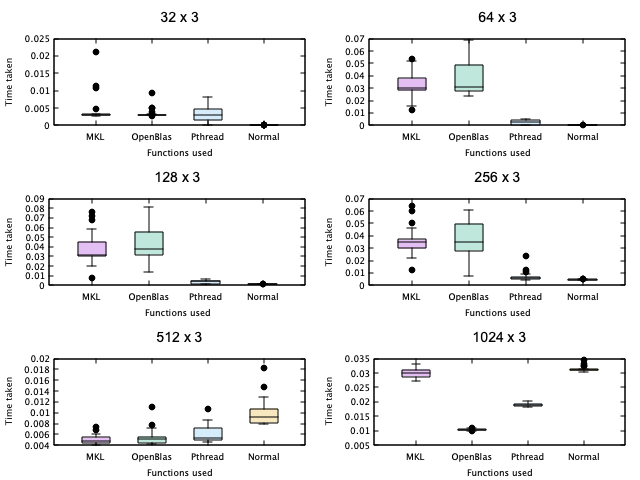
\includegraphics[width=10cm]{3filter.png}
\end{center}
\caption{Box plots for all 4 implementation for all filters and input matrix} \label{3filter}
\end{figure}


While figure \ref{9filter} shows the dependence for filter size of 9.

\begin{figure}[!htbp]
\begin{center}
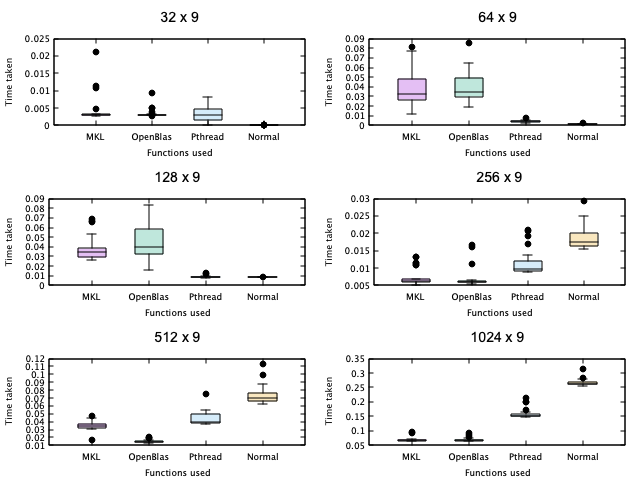
\includegraphics[width=12cm]{9filter.png}
\end{center}
\caption{Box plots for all 4 implementation for all filters and input matrix} \label{9filter}
\end{figure}

\section{Conclusions}

After implementing each of the above models, we see that for small values of filter sizes, normal multiplication and pthread are the fastest (pthread is the faster of the two), and as we increase the sizes MKL and OpenBlas become the fastest with OpenBlas a tad faster than MKL.



\bibliographystyle{plain}
\bibliography{bibliography.bib}
\end{document}